\section[光子]{\makebox[5em][s]{光子}}\label{sec:01.02}
% \makebox[5em][s]{} % 短题目拉间距
% \setlength{\mathindent}{9em} 本文标准公式缩进

1905年,爱因斯坦将普朗克的量子假设发展成光量子(光子)的概念也正是这一年,爱因斯坦创立了狭义相对论.

爱因斯坦认为,电磁波(光波)的结构应该是量子化的,其最小单元即一个光子,每个光子均以同样的速度$c$(光速)运动频率为$v$的光波,其光子的能量和动量为
\begin{align}
	E=h\nu=\hbar\omega \label{eqn:01.02.01} \\ 
	p\approx \frac{E}{c}=\frac{h\nu}{c}=\frac{h}{\lambda} \label{eqn:01.02.02}
\end{align}
$\lambda$为光波的波长,光子的运动方向应该和光波的传播方向一致.

对于单色平面波,如引入“波矢量”$\boldsymbol{k}$,其方向为波的传播方向,其数值为$k=| \boldsymbol{k}|=\frac{2\pi}{\lambda}$,则光子的动量可以表示成
\eqindent{12}
\begin{equation}\label{eqn:01.02.03}
	\boldsymbol{p}=\hbar \boldsymbol{k}
\end{equation}\eqnormal

光和其他物质发生相互作用时,基元过程通常表现为光子-电子作用或者光子-原子作用,利用光子的概念并对作用过程应用能量守恒定律,一般就能够得出某些(但不是全部)重要结论.

\textsf{1. 光电效应}

某些金属受到光的照射后,能够发射出电子,形成电流,这就是光电效应其物理机理可用光子概念解释如下金属中的“自由电子”要逸出金属表面,需要克服“逸出功”,$W$当金属受到频率为$v$的光照射时,自由电子即可吸收光子,从而获得能量(电子同时或在短时间内连续吸收两个以上光子的机会极小,可以不考虑这种可能性.)如$h\nu>W$,电子就可以从金属中逸出,并具有动能
\begin{equation}\label{eqn:01.02.04}
	\boxed{\frac{1}{2}m_{c}v^{2}=h\nu-W}
\end{equation}
由此可见,光电子的动能完全由逸出功$W$(由金属性质决定)和入射光的频率$v$所决定,而与光的强度无关光电子的数目则与入射光的强度成正比,即和入射光子的总数成正比对光电子动能的实验测量完全证实了爱因斯坦公式\eqref{eqn:01.02.04}的正确性由\eqref{eqn:01.02.04}式还可看出,当逸出功$W$给定后,入射光的频率$v$必须超过$W/h$,才能产生光电效应;如$v<\frac{W}{h}$,尽管光很强,也不会产生光电子这个结论也已为实验证实.

\textsf{2. 康普顿散射}

关于光子能量和动量的爱因斯坦公式\eqref{eqn:01.02.01}、\eqref{eqn:01.02.03},于l923年被康普顿(A.H.Compton)散射所证实实验发现,X射线被石蜡等轻物质散射时,波长增大经典电磁理论很难解释这现象康普顿利用光子的概念,并假定在光子-电子作用过程中,能量守恒定律和动量守恒定律成立,利用相对论力学,对散射过程作出了成功的理论分析.

$X$射线的光子能量,约在$10^{3}\si{eV}$以上轻物质中外层电子的原子能级仅几个电子伏,可以当作自由电子设$X$射线的入射波长为$\lambda$,则入射光子的能量、动量为
\begin{equation} 
	\begin{aligned} \notag
		E=h\nu=\frac{hc}{\lambda} \\
		p=\frac{E}{c}=\frac{h\nu}{c}=\frac{h}{\lambda}
	\end{aligned}
\end{equation}
\begin{wrapfigure}[7]{r}{9em}
	\centering
	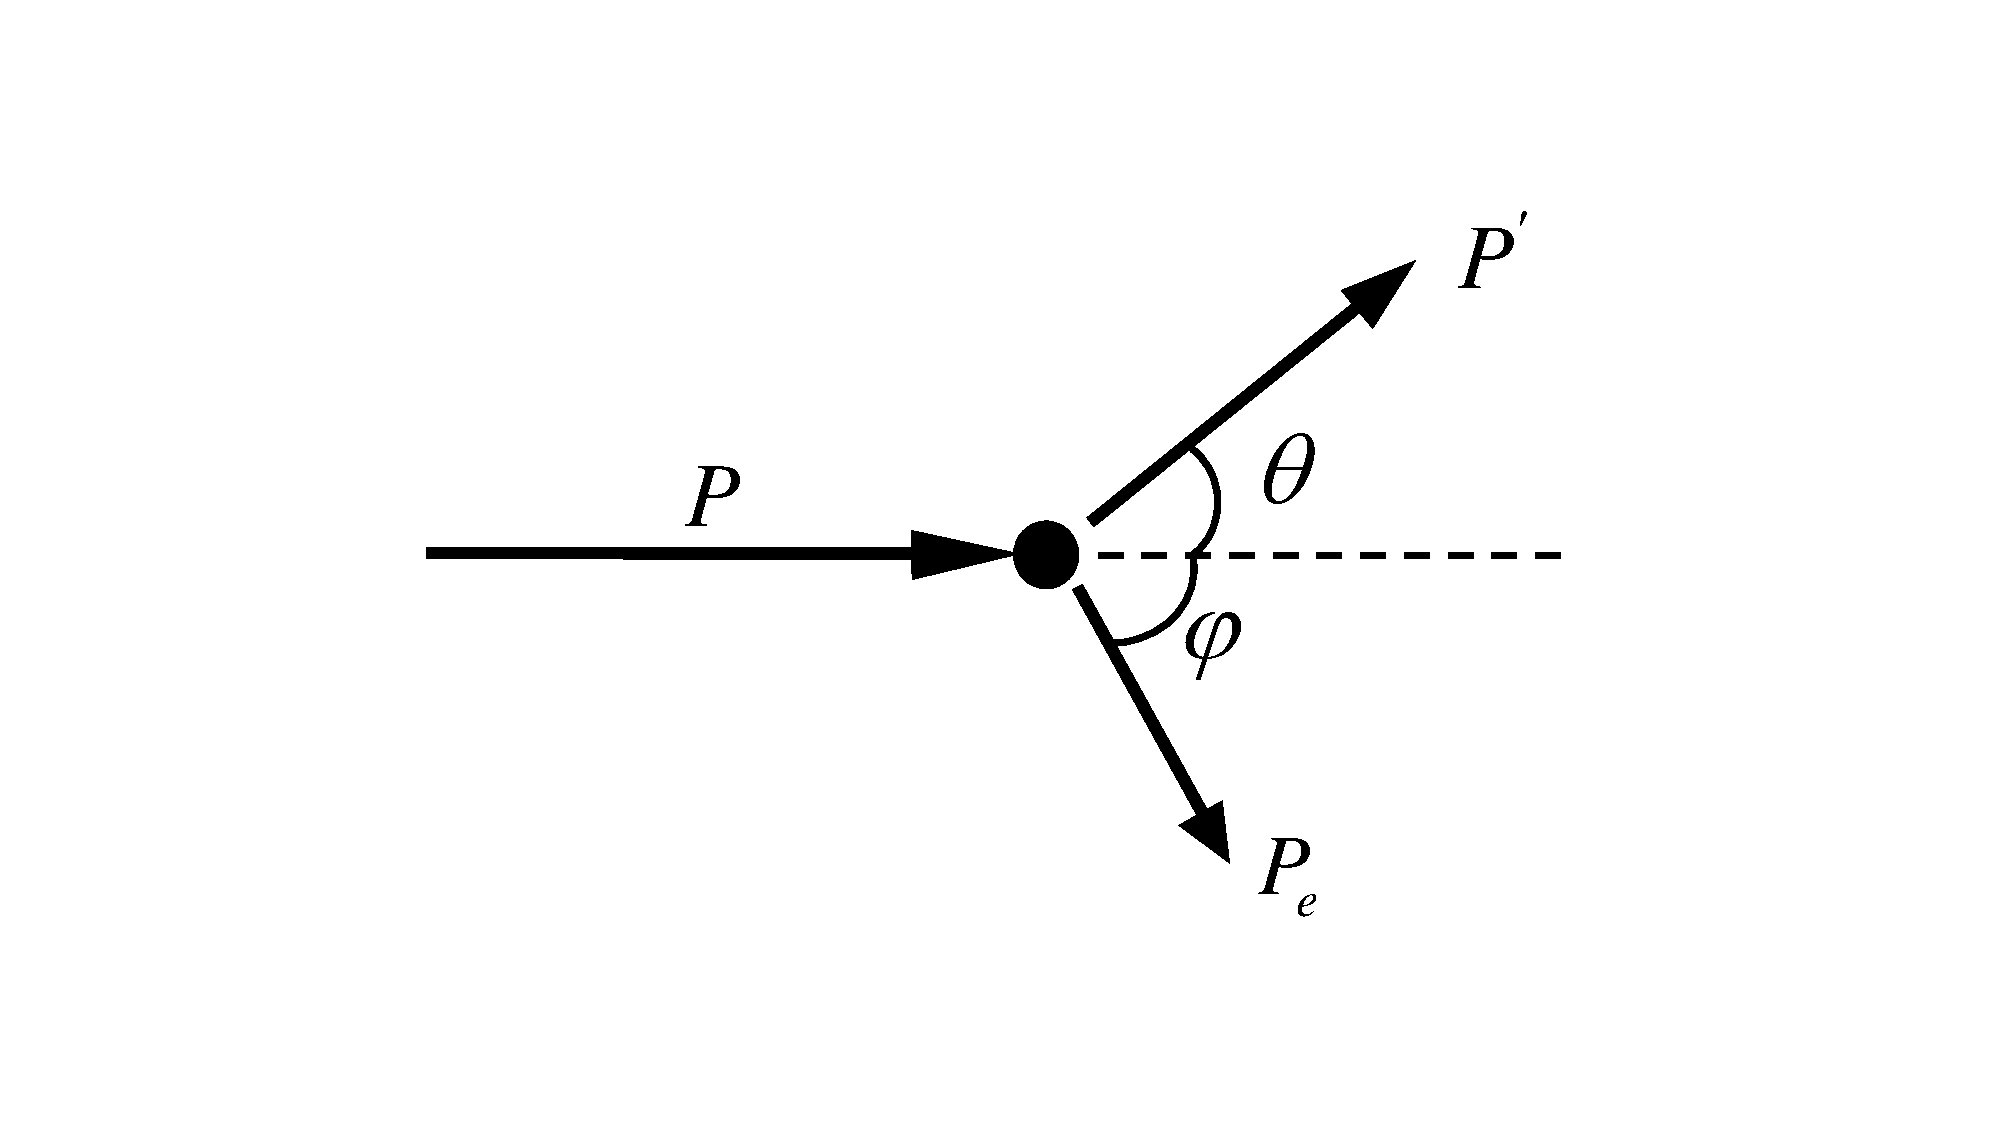
\includegraphics[width=3cm]{QM file/figure/1-3}
	\caption{}
	\label{fig.1-3}
\end{wrapfigure}
电子初始动量为0,初始能量为$m_{c}c^{2}$散射(碰撞)后,设光子沿$\theta$方向射出,如图\ref{fig.1-3},波长变为$\lambda^{\prime}$,能量及动量变为
\setlength{\mathindent}{6em}
\begin{equation}
	\begin{aligned} \notag
		E^{\prime}=h\nu^{\prime}=\frac{hc}{\lambda^{\prime}} \\
		p^{\prime}=\frac{E^{\prime}}{c}=\frac{h\nu^{\prime}}{c}=\frac{h}{\lambda^{\prime}}
	\end{aligned}
\end{equation}
\eqnormal
电子的反冲角设为$\varphi$能量和动量设为$E_{e}$和$p_{e}$,按照相对论力学
\begin{equation}\label{eqn:01.02.05}
	E_{e}^2=c^{2}p_{e}^{2}+m_{e}^{2}c^{4}
\end{equation}
对散射过程应用能量守恒定律,得到
\begin{equation*}
	h\nu+m_{e}c^{2}=h\nu^{\prime}+E_{e}^{2}
\end{equation*}
亦即
\begin{equation}\label{eqn:01.02.06}
	h(\nu-\nu^{\prime})=E_{e}-m_{e}c^{2}
\end{equation}
对散射过程应用动量守恒定律,得到
\begin{equation}\label{eqn:01.02.07}
	\boldmath p-p^{\prime}=p_{e}
\end{equation}
取平方,得到
\begin{equation*}
	p^{2}+p^{\prime 2}-2\boldsymbol{p}\cdot\boldsymbol{p^{\prime}}=p_{e}^{2}
\end{equation*}
亦即
\begin{equation}\label{eqn:01.02.08}
	h^{2}(\nu+\nu^{\prime}-2\nu\nu^{\prime}\cos\theta)=E_{e}^{2}-m_{e}^{2}c^{4}
\end{equation}
\eqref{eqn:01.02.06}式取平方,则得
\begin{equation*}
	h^{2}(\nu+\nu^{\prime}-2v\nu^{\prime})=(E_{e}-m_{e}c^{2})^{2}
\end{equation*}
与\eqref{eqn:01.02.08}式相消,得到
\begin{equation}
	\begin{aligned}
		2h^{2}\nu\nu^{\prime}(1-\cos\theta) &=2m_{e}c^{2}(E_{e}-m_{e}c^{2}) \\
		&=2m_{e}c^{2}h(\nu-\nu^{\prime})
	\end{aligned}
\end{equation}
因此,
\begin{equation*}
	\frac{1}{\nu}-\frac{1}{\nu^{\prime}}=\frac{h}{m_{e}c^{2}}(1-\cos\theta)
\end{equation*}
亦即
\begin{equation}\label{eqn:01.02.09}
	\boxed{\lambda^{\prime}-\lambda=\frac{h}{m_{e}c}(1-\cos\theta)}
\end{equation}
经过散射,X射线得波长有所增加,增量$(\lambda^{\prime}-\lambda)$与散射角有关,并与$\frac{h}{m_{e}c}$成比例,后者称为康普顿波长,记为$\lambda_{c}$,
\begin{equation}\label{eqn:01.02.10}
	\lambda_{c}=\frac{h}{m_{e}c}=2.43\times10^{-12} \si{m}
\end{equation}
对散射光波长的实验证实了\eqref{eqn:01.02.09}式的正确性因此,康普顿散射证实了:(i)光子的能量、动量公式\eqref{eqn:01.02.01}、\eqref{eqn:01.02.02}、\eqref{eqn:01.02.03}是正确的;(ii)微观基元过程中,能量守恒定律和动量守恒定律成立;(iii)相对论力学是正确的.

\textsf{3. 粒子-反粒子对的湮没与产生}

实验发现,电子($e^{-}$)及其反粒子(正电子,$e^{+}$)相碰,可以湮没而产生两个$\gamma$光子,即
\begin{equation*}
	e^{-}+e^{+}\rightarrow \gamma+\gamma
\end{equation*}
根据相对论力学及能量、动量守恒定律,每个$\gamma$光子的能量至少等于电子的静能,即$E_{r}\geqslant m_{e}c^{2}$,相应的$\gamma$射线波长为
\begin{equation*}
	\lambda=\frac{hc}{E_{r}}\leqslant\frac{h}{m_{e}c}=\lambda_{c}
\end{equation*}
这个关系已为实验所证实粒子物理的理论分析表明,能够产生上述湮没过程的电子、正电子距离,大致也是康普顿波长的量级.

在温度$T$下,热辐射光子的平均能量约为$3kT$(k为玻尔兹曼常数)按照近代天体物理理论,在宇宙形成的初期,温度极高,两个光子相碰,可能转变成(质子、反质子)对或(中子,反中子)对,按照能量守恒定律,有
\begin{equation*}
	E_{\gamma}\approx3kT\approx m_{p}c^{2}=938 \si{MeV}
\end{equation*}
因此当时温度约为
\begin{equation*}
	T\approx m_{p}c^{2} \big/ 3k\approx3.6\times10^{12} \si{K}
\end{equation*}


